%-----------------------------------------------------------------------------------------------------------------------------------------------%
%	The MIT License (MIT)
%
%	Copyright (c) 2019 Jan Küster
%
%	Permission is hereby granted, free of charge, to any person obtaining a copy
%	of this software and associated documentation files (the "Software"), to deal
%	in the Software without restriction, including without limitation the rights
%	to use, copy, modify, merge, publish, distribute, sublicense, and/or sell
%	copies of the Software, and to permit persons to whom the Software is
%	furnished to do so, subject to the following conditions:
%	
%	THE SOFTWARE IS PROVIDED "AS IS", WITHOUT WARRANTY OF ANY KIND, EXPRESS OR
%	IMPLIED, INCLUDING BUT NOT LIMITED TO THE WARRANTIES OF MERCHANTABILITY,
%	FITNESS FOR A PARTICULAR PURPOSE AND NONINFRINGEMENT. IN NO EVENT SHALL THE
%	AUTHORS OR COPYRIGHT HOLDERS BE LIABLE FOR ANY CLAIM, DAMAGES OR OTHER
%	LIABILITY, WHETHER IN AN ACTION OF CONTRACT, TORT OR OTHERWISE, ARISING FROM,
%	OUT OF OR IN CONNECTION WITH THE SOFTWARE OR THE USE OR OTHER DEALINGS IN
%	THE SOFTWARE.
%	
%
%-----------------------------------------------------------------------------------------------------------------------------------------------%


%============================================================================%
%
%	DOCUMENT DEFINITION
%
%============================================================================%

%we use article class because we want to fully customize the page and don't use a cv template
\documentclass[10pt,A4]{article}	


%----------------------------------------------------------------------------------------
%	ENCODING
%----------------------------------------------------------------------------------------

% we use utf8 since we want to build from any machine
\usepackage[utf8]{inputenc}		

%----------------------------------------------------------------------------------------
%	LOGIC
%----------------------------------------------------------------------------------------

% provides \isempty test
\usepackage{xstring, xifthen}

%----------------------------------------------------------------------------------------
%	FONT BASICS
%----------------------------------------------------------------------------------------

% some tex-live fonts - choose your own

%\usepackage[defaultsans]{droidsans}
%\usepackage[default]{comfortaa}
%\usepackage{cmbright}
\usepackage[default]{raleway}
%\usepackage{fetamont}
%\usepackage[default]{gillius}
%\usepackage[light,math]{iwona}
%\usepackage[thin]{roboto} 

% set font default
\renewcommand*\familydefault{\sfdefault} 	
\usepackage[T1]{fontenc}

% more font size definitions
\usepackage{moresize}

%----------------------------------------------------------------------------------------
%	FONT AWESOME ICONS
%---------------------------------------------------------------------------------------- 

% include the fontawesome icon set
\usepackage{fontawesome}

% use to vertically center content
% credits to: http://tex.stackexchange.com/questions/7219/how-to-vertically-center-two-images-next-to-each-other
\newcommand{\vcenteredinclude}[1]{\begingroup
\setbox0=\hbox{\includegraphics{#1}}%
\parbox{\wd0}{\box0}\endgroup}

% use to vertically center content
% credits to: http://tex.stackexchange.com/questions/7219/how-to-vertically-center-two-images-next-to-each-other
\newcommand*{\vcenteredhbox}[1]{\begingroup
\setbox0=\hbox{#1}\parbox{\wd0}{\box0}\endgroup}

% icon shortcut
\newcommand{\icon}[3] { 							
	\makebox(#2, #2){\textcolor{maincol}{\csname fa#1\endcsname}}
}	

% icon with text shortcut
\newcommand{\icontext}[4]{ 						
	\vcenteredhbox{\icon{#1}{#2}{#3}}  \hspace{2pt}  \parbox{0.9\mpwidth}{\textcolor{#4}{#3}}
}

% icon with website url
\newcommand{\iconhref}[5]{ 						
    \vcenteredhbox{\icon{#1}{#2}{#5}}  \hspace{2pt} \href{#4}{\textcolor{#5}{#3}}
}

% icon with email link
\newcommand{\iconemail}[5]{ 						
    \vcenteredhbox{\icon{#1}{#2}{#5}}  \hspace{2pt} \href{mailto:#4}{\textcolor{#5}{#3}}
}

%----------------------------------------------------------------------------------------
%	PAGE LAYOUT  DEFINITIONS
%----------------------------------------------------------------------------------------

% page outer frames (debug-only)
% \usepackage{showframe}		

% we use paracol to display breakable two columns
\usepackage{paracol}

% define page styles using geometry
\usepackage[a4paper]{geometry}

% remove all possible margins
\geometry{top=1cm, bottom=1cm, left=1cm, right=1cm}

\usepackage{fancyhdr}
\pagestyle{empty}

% space between header and content
% \setlength{\headheight}{0pt}

% indentation is zero
\setlength{\parindent}{0mm}

%----------------------------------------------------------------------------------------
%	TABLE /ARRAY DEFINITIONS
%---------------------------------------------------------------------------------------- 

% extended aligning of tabular cells
\usepackage{array}

% custom column right-align with fixed width
% use like p{size} but via x{size}
\newcolumntype{x}[1]{%
>{\raggedleft\hspace{0pt}}p{#1}}%


%----------------------------------------------------------------------------------------
%	GRAPHICS DEFINITIONS
%---------------------------------------------------------------------------------------- 

%for header image
\usepackage{graphicx}

% use this for floating figures
% \usepackage{wrapfig}
% \usepackage{float}
% \floatstyle{boxed} 
% \restylefloat{figure}

%for drawing graphics		
\usepackage{tikz}				
\usetikzlibrary{shapes, backgrounds,mindmap, trees}

%----------------------------------------------------------------------------------------
%	Color DEFINITIONS
%---------------------------------------------------------------------------------------- 
\usepackage{transparent}
\usepackage{color}

% primary color
\definecolor{maincol}{RGB}{ 203, 23, 23}
%\definecolor{maincol}{RGB}{0,128,0}

% accent color, secondary
% \definecolor{accentcol}{RGB}{ 250, 150, 10 }

% dark color
\definecolor{darkcol}{RGB}{ 70, 70, 70 }

% light color
\definecolor{lightcol}{RGB}{245,245,245}


% Package for links, must be the last package used
\usepackage[hidelinks]{hyperref}

% returns minipage width minus two times \fboxsep
% to keep padding included in width calculations
% can also be used for other boxes / environments
\newcommand{\mpwidth}{\linewidth-\fboxsep-\fboxsep}
	


%============================================================================%
%
%	CV COMMANDS
%
%============================================================================%

%----------------------------------------------------------------------------------------
%	 CV LIST
%----------------------------------------------------------------------------------------

% renders a standard latex list but abstracts away the environment definition (begin/end)
\newcommand{\cvlist}[1] {
  \begin{itemize}
    \setlength{\itemsep}{2pt} % Riduci lo spazio tra gli elementi
    \setlength{\topsep}{0pt} % Riduci lo spazio prima di un elemento
    #1
  \end{itemize}
}

%----------------------------------------------------------------------------------------
%	 CV TEXT
%----------------------------------------------------------------------------------------

% base class to wrap any text based stuff here. Renders like a paragraph.
% Allows complex commands to be passed, too.
% param 1: *any
\newcommand{\cvtext}[1] {
	\begin{tabular*}{1\mpwidth}{p{0.98\mpwidth}}
		\parbox{1\mpwidth}{#1}
	\end{tabular*}
}

%----------------------------------------------------------------------------------------
%	CV SECTION
%----------------------------------------------------------------------------------------

% Renders a a CV section headline with a nice underline in main color.
% param 1: section title
\newcommand{\cvsection}[1] {
	\vspace{14pt}
	\cvtext{
		\textbf{\LARGE{\textcolor{darkcol}{\uppercase{#1}}}}\\[-4pt]
		\textcolor{maincol}{ \rule{0.1\textwidth}{2pt} } \\
	}
}

%----------------------------------------------------------------------------------------
%	META SKILL
%----------------------------------------------------------------------------------------

% Renders a progress-bar to indicate a certain skill in percent.
% param 1: name of the skill / tech / etc.
% param 2: level (for example in years)
% param 3: percent, values range from 0 to 1
\newcommand{\cvskill}[3] {
	\begin{tabular*}{1\mpwidth}{p{0.72\mpwidth}  r}
 		\textcolor{black}{\textbf{#1}} %& \textcolor{maincol}{#2}%\\
	\end{tabular*}%
	
	\hspace{4pt}
	\begin{tikzpicture}[scale=1,rounded corners=2pt,very thin]
		\fill [lightcol] (0,0) rectangle (1\mpwidth, 0.15);
		\fill [maincol] (0,0) rectangle (#3\mpwidth, 0.15);
  	\end{tikzpicture}%
}


%----------------------------------------------------------------------------------------
%	 CV EVENT
%----------------------------------------------------------------------------------------

\newcommand{\cvevent}[7] {
    \ifthenelse{\value{eventcount}>0}{\vspace{4pt} \noindent\textcolor{lightcol}{\rule{\linewidth}{0.5pt}} \vspace{10pt}}{}
    \stepcounter{eventcount}

    \parbox{\mpwidth}{
        \begin{tabular*}{1\mpwidth}{p{0.72\mpwidth} r}
            \raggedright\textcolor{black}{\textbf{#2}} & 
            \textbf{\underline{\textcolor{black}{#1}}} \\
            \raggedright\textcolor{maincol}{\textbf{#3}} & \\
        \end{tabular*}\\[6pt]

        \ifthenelse{\isempty{#4}}{}{
            \cvtext{#4}\\
        }
    }

    \ifthenelse{\isempty{#5}}{}{
        \vspace{4pt}
        {#5}
    }
    
    \parbox{\mpwidth}{
    \ifthenelse{\isempty{#6}}{}{
        \vspace{4pt}
        \cvtext{\textbf{Technologies include:}}%\\
        {#6}
    }
    }

    \parbox{\mpwidth}{
    \ifthenelse{\isempty{#7}}{}{
        \vspace{4pt}
        \cvtext{\textbf{Achievements include:}}%\\
        {#7}
    }
    }
    
    \vspace{4pt}
}

%----------------------------------------------------------------------------------------
%	 CV META EVENT
%----------------------------------------------------------------------------------------

% Renders a CV event on the sidebar
% param 1: title
% param 2: subtitle (optional)
% param 3: customer, employer, etc,. (optional)
% param 4: info text (optional)
\newcommand{\cvmetaevent}[4] {
	\textcolor{maincol} {\cvtext{\textbf{\begin{flushleft}#1\end{flushleft}}}}

	\ifthenelse{\isempty{#2}}{}{
	\textcolor{darkcol} {\cvtext{\textbf{#2}} }
	}

	\ifthenelse{\isempty{#3}}{}{
		\cvtext{{ \textcolor{darkcol} {#3} }}\\
	}

	\cvtext{#4}\\[14pt]
}

%---------------------------------------------------------------------------------------
%	QR CODE
%----------------------------------------------------------------------------------------

% Renders a qrcode image (centered, relative to the parentwidth)
% param 1: percent width, from 0 to 1
\newcommand{\cvqrcode}[1] {
	\begin{center}
		\includegraphics[width={#1}\mpwidth]{qrcode}
	\end{center}
}


%============================================================================%
%
%
%
%	DOCUMENT CONTENT
%
%
%
%============================================================================%
\begin{document}
\newcounter{eventcount}
\setcounter{eventcount}{0}
\columnratio{0.31}
\setlength{\columnsep}{2.2em}
\setlength{\columnseprule}{4pt}
\colseprulecolor{lightcol}
\begin{paracol}{2}
\begin{leftcolumn}
%---------------------------------------------------------------------------------------
%	META IMAGE
%----------------------------------------------------------------------------------------
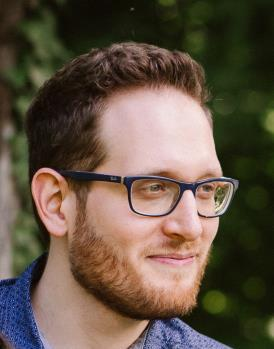
\includegraphics[width=\linewidth]{profile.jpg}	%trimming relative to image size

%---------------------------------------------------------------------------------------
%	META SKILLS
%----------------------------------------------------------------------------------------
\cvsection{SKILLS}

\cvskill{Java} {10+ yrs} {1.0} \\[-2pt]
\cvskill{Linux} {10+ yrs} {1.0} \\[-2pt]
\cvskill{Scala} {5+ yrs} {0.9} \\[-2pt]
\cvskill{Spring Framework} {10+ yrs} {0.9} \\[-2pt]
\cvskill{C++} {3+ yrs} {0.8} \\[-2pt]
\cvskill{Typescript} {5+ yrs} {0.8} \\[-2pt]
\cvskill{ROS2} {2+ yrs} {0.7} \\[-2pt]
\cvskill{Python} {3+ yrs} {0.7} \\[-2pt]

\vspace{10pt}
\cvskill{Teamwork} {10+ yrs} {1.0} \\[-2pt]
\cvskill{Problem-solving} {10+ yrs} {0.9} \\[-2pt]
\cvskill{Mentoring} {10+ yrs} {0.9} \\[-2pt]
\cvskill{Leadership} {5+ yrs} {0.9} \\[-2pt]
\cvskill{Decision-making} {5+ yrs} {0.8} \\[-2pt]
\cvskill{Innovation} {10+ yrs} {0.8} \\[-2pt]
\cvskill{Communication} {2+ yrs} {0.7} \\[-2pt]
\cvskill{Negotiation} {2+ yrs} {0.6} \\[-2pt]


%\vfill\null
\cvsection{CONTACT}

\icontext{MapMarker}{12}{Avigliana (TO), Italy}{black}\\[6pt]
\icontext{MobilePhone}{12}{338-9904630}{black}\\[6pt]
\iconemail{Envelope}{12}{danieleb88@gmail.com}{danieleb88@gmail.com}{black}\\[6pt]
\iconhref{Github}{12}{github.com/dbortoluzzi}{https://github.com/dbortoluzzi}{black}\\[6pt]
%\iconhref{Orcid}{12}{0009-0004-2056-9111}{https://orcid.org/0009-0004-2056-9111}{black}\\[6pt]

\vfill\null


%---------------------------------------------------------------------------------------
%	EDUCATION
%----------------------------------------------------------------------------------------
\newpage
\cvsection{EDUCATION}

\cvmetaevent
{09/2013 -- 07/2022}
{Master's Degree in Computer Science (Level 7 EQF)}
{University of Turin}
{Graduation grade: \emph{110/110 with honors and dignity of printing}.}

\cvmetaevent
{09/2007 -- 06/2011}
{Bachelor's Degree in Computer Science (Level 6 EQF)}
{Ca' Foscari University of Venice}
{Graduation grade: \emph{104/110}.}

\cvmetaevent
{09/2002 -- 06/2007}
{Scientific High School Diploma}
{Liceo Scientifico Statale “G. Marconi” di Conegliano (TV)}
{National Plan for Informatics.\\
Final grade: 90/100.}

%\vfill\null


%---------------------------------------------------------------------------------------
%	CERTIFICATIONS
%----------------------------------------------------------------------------------------
%\newpage
%\cvsection{CERTIFICATIONS}
%% -- Add your certifications here if needed --

%\vfill

%---------------------------------------------------------------------------------------
%	PUBLICATIONS
%----------------------------------------------------------------------------------------

\cvsection{PUBLICATIONS}

\cvtext{
\textbf{A. Basso, D. Bortoluzzi, G.Torta, D. Pau, L. Chariglione, F. Damiani.} \\
"Architecture standardization for AI deployment on tiny micro-controllers", \\
Proc. of the 12th IEEE Int. Conf. on Consumer Technology, 2-6 September 2022, Berlin (Germany)
}

\vspace{10pt}

\cvtext{
\textbf{A. Basso, D. Bortoluzzi and G. Torta.} \\
"Implementation of an IoT Wearable Prototype on a Standard AI Architecture," 2022 IEEE Intl Conf on Dependable, Autonomic and Secure Computing, Intl Conf on Pervasive Intelligence and Computing, Intl Conf on Cloud and Big Data Computing, Intl Conf on Cyber Science and Technology Congress (DASC / PiCom / CBDCom / CyberSciTech), Falerna, Italy, 2022, pp. 1-5
}

\vspace{10pt}

\cvtext{
\textbf{Audrito, G., Bortoluzzi, D., Damiani, F., Scarso, G., Torta, G.} \\
"An Enhanced Exchange Operator for XC." In: Castellani, I., Tiezzi, F. (eds) Coordination Models and Languages. COORDINATION 2024. Lecture Notes in Computer Science, vol 14676. Springer, Cham
}

\vfill


\end{leftcolumn}
\begin{rightcolumn}
%---------------------------------------------------------------------------------------
%	TITLE  HEADER
%----------------------------------------------------------------------------------------
\fcolorbox{white}{darkcol}{\begin{minipage}[c][3.5cm][c]{1\mpwidth}
	\begin {center}
		\HUGE{ \textbf{ \textcolor{white}{ \uppercase{DANIELE BORTOLUZZI} } } } \\[-24pt]
		\textcolor{white}{ \rule{0.1\textwidth}{1.25pt} } \\[4pt]
		\large{ \textcolor{white} {Software and IoT Architect / R\&D} }
	\end {center}
\end{minipage}} \\[14pt]
\vspace{-12pt}

%---------------------------------------------------------------------------------------
%	PROFILE
%----------------------------------------------------------------------------------------
%\vfill\null
\vspace{8pt}
\cvsection{PROFILE}

\cvtext{I'm a computer scientist with 15 years of professional experience and a passion for IT and new technologies. I specialize in developing architectures and frameworks using Java and Python. My research focuses on swarm robotics and the Internet of Things (IoT), designing and implementing solutions for \emph{embedded devices}, \emph{rovers}, \emph{robots}, and \emph{drones}.}

%---------------------------------------------------------------------------------------
%	WORK EXPERIENCE
%----------------------------------------------------------------------------------------
\vspace{16pt}
\cvsection{WORK EXPERIENCE}

\cvevent
{03/2023 -- now}
{Research Fellow}
{University of Turin, Department of Computer Science}
{Within the MoVeRe research group at the University of Turin, I conduct research activities related to the \underline{Aggregate Programming} paradigm, which allows leveraging \underline{coordination} between heterogeneous entities.}
{\cvlist{
	\item Participation in the PRIN 2020 project named \underline{COMMON-WEARS}.
	\item Collaboration in the organization and development of verticalizations and PoC in the \underline{Smart Mobility} and \underline{Industry 4.0} sectors.
	\item Teaching support activities for the courses “Web Technologies” and “Programming for mobile devices”.
}}
{\cvlist{
	\item \underline{ROS2} (Python, C++), \underline{Gazebo} (Python), Zephyr (C, C++), Arduino (C), Spring Boot (Java), Angular (Typescript).
}}
{\cvlist{
	\item A new \underline{platform} for IoT and robotics using Aggregate Programming and ROS2.
	\item Working on \underline{PRIN and European projects}, using R\&D tecnology in specialized industry.
	\item Published some research papers related to Aggregate Programming.
}}


\cvevent
{10/2021 -- 03/2023}
{Solution Architect}
{GFT Italia S.r.l. (Turin)}
{Consulting activities in software architectural analysis and design for microservices for insurance market clients.}
{\cvlist{
	\item Technical reference and coordination of development teams.
	\item Technical training and coaching activities for resources.
	\item Design and coordination of the IT solution for the new core customer registry system for a lead insurance group.
}}
{\cvlist{
	\item \underline{Java 11+}, \underline{Spring Boot}, \underline{Oracle}, Spring Cloud, Redis, DB2, MyBatis, Tomcat, IBM WebSphere, SQL, Gitlab, Maven, REST, IBM MQ, Apache Kafka.
}}
{\cvlist{
	\item Managed and detailed complex systems for \underline{enterprise-level} projects.
	\item \underline{Led} a team of 20+ members, with different roles and skill-set.
}}

%\vfill\null
\cvevent
{01/2017 -- 10/2021}
{Senior Software Developer / Technical Leader}
{Xeffe S.r.l. (Turin)}
{Analysis, coordination, and development of Enterprise Solutions for the finance market.}
{\cvlist{
	\item Use of Domain Driven Design and Enterprise Integration Patterns.
	\item Development and maintenance of projects for finance market.
	\item Development and maintenance of proprietary frameworks based on Apache Camel and Play Framework.
}}
{\cvlist{
	\item \underline{Java 8+}, \underline{Scala}, \underline{Javascript}, Spring, SQL, Apache Camel, Play Framework, Oracle, H2, MyBatis, GitHub, Ansible, Maven, nginx, SOAP, REST, JQuery, BeanIO, Quartz.
}}
{\cvlist{
	\item High customer satisfaction in the design and implementation of \underline{customer-specific projects} using proprietary frameworks.
}}

%\vfill\null
\cvevent
{06/2015 -- 01/2017}
{Software Architect / Full Stack Developer}
{Audacia S.r.l. (Turin)}
{Coordination and development of an Intelligent Big Data Analysis system to extract significant information from heterogeneous data sources.}
{\cvlist{
	\item Analysis and development of software solutions for insurance companies.
	\item Mantainance of Java applications for finance market.
}}
{\cvlist{
	\item \underline{Node.js}, \underline{Google Cloud Platform}, \underline{Javascript}, \underline{ArangoDB}, Java, SQL, AQL, Loopback, Express, AngularJS, Oracle, GitHub, GIT, Grunt, Bower, NPM, Bootstrap.
}}
{\cvlist{
	\item Implemented a \underline{draft solution} for Intelligent Big Data Analysis using \underline{cutting-edge} technologies.
}}

%\vfill\null
\cvevent
{11/2014 -- 06/2015}
{Software Engineer / IT Manager}
{Creatiweb S.r.l. (Turin)}
{Fullstack development of a proprietary booking engine for campsites and villages}
{\cvlist{
	\item Development of WebServices to integrate the booking engine with accounting and channel manager software.
	\item Implementation of new features of the booking engine application.
	\item Performance analysis and tuning of company databases.
	\item Manager of the server farm.
}}
{\cvlist{
	\item \underline{Java}, \underline{SQL}, \underline{Linux}, \underline{Javascript}, PHP, XSD, XML, CSS, HTML, SQL, Bash Script, Firebird DBMS, Tomcat, JQuery, XPath, XMLBeans, SOAP.
}}
{\cvlist{
	\item Served as the main point of contact for the IT department, supporting both internal and external clients.
}}

%\vfill\null
\cvevent
{11/2011 -- 11/2014}
{Software Engineer / Developer}
{NaturalBooking S.r.l. (Turin)}
{Development of the back-end of Hospes, a booking engine used by a lot of campsites and villages in Italy.}
{\cvlist{
	\item Development of SOAP WebServices to integrate the Booking Engine with accounting and channel manager software.
	\item IT administration of servers hosting the application.
}}
{\cvlist{
	\item \underline{Java}, \underline{Firebird DBMS}, Javascript, SQL, XML, CSS, HTML, Bash Script, Tomcat, SOAP.
}}
{}

%\vfill\null
\cvevent
{06/2011 -- 11/2011}
{Analyst / Developer}
{Prosa S.r.l. (Venice)}
{Implementation of server-side and client-side features of the EmotiVending system, a vending machine equipped with a touch multimedia interface.}
{\cvlist{
	\item Analysis and development of the new VeBox system, a control center for vending machine controllers, in Java.
	\item Development of an application for testing hardware of vending machines.
}}
{\cvlist{
	\item \underline{C++}, \underline{Ruby}, Java, Linux, Tomcat, Java Swing, Restlet.
}}
{}


% hotfixes to create fake-space to ensure the whole height is used
\mbox{}
\vfill

\mbox{}
\vfill

\mbox{}
\vfill

\mbox{}

\end{rightcolumn}
\end{paracol}

\vfill
\noindent \emph{I authorize the processing of my personal data pursuant to Legislative Decree 196/2003 and the GDPR (EU Regulation 2016/679) for recruitment purposes.}

\end{document}
